
\subsection{Algoritmi di ordinamento privi di confronti}

\subsubsection{CountingSort}

{{[}CLRS{]} pp. 159-161}

{Assunzione:}

{~~~~~~~~I numeri da ordinare sono interi in un intervallo che va da 0 a $k$, per qualche $k$ prefissato}

{Input:}

{$A=[0,\ldots,n]$ dove $A[j] \in [0,\ldots,k]$, $n,k$ sono parametri}

{Output:}

{$B=[0,\ldots,n]$ ordinato, permutazione di A}

{Utilizzo una memoria ausiliaria $C$, costituita da $k+1$ elementi, $C=[0,\ldots,n]$}

{Codice:}

\lstinputlisting{code/counting_sort.txt}

{Complessità di CountingSort : $\Theta(n+k)$}

{Di solito il CountingSort quando $k$ è limitato superiormente da n, $k=O(n)$. Allora il tempo di esecuzione risulta $\Theta(n)$. Il tempo di esecuzione di questo algoritmo è dato da
$\Theta(n+k)$. Il CountingSort di solito è utilizzato quando $k$ è limitato superiormente da $n$ in $k=O(n)$. Allora, il tempo di esecuzione risulta essere $O(n)$.}

{Il CountingSort è un algoritmo stabile, caratteristica molto importante.}

{Analisi:}

{~~~~~~~~All'uscita dal secondo ciclo: $C[i] = \abs{\{x \in \{1\ldots n\}\,|\,A[x] = i\}}$}

{~~~~~~~~All'uscita dal terzo giro: $C[i] = \abs{\{x \in \{1\ldots n\}\,|\,A[x] \leq i\}}$}


\subsubsection{RadixSort}

{{[}CLRS{]} pp. 162-164}

{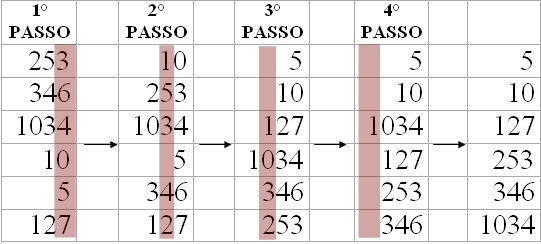
\includegraphics{images/image540.png}}

{L'algoritmo di ordinamento scelto deve essere stabili e rispettare l'ordine.}

\lstinputlisting{code/radix_sort.txt}

{Dimostriamo la correttezza dell'algoritmo tramite induzione sulla colonna da ordinare:}

{Caso base (i=1)}

{~~~~~~~~Ordino l'unica colonna}

{Assumo che le cifre delle colonne che vanno da $1$ a $i-1$ siano ordinate}

{Dimostro che un algoritmo stabile sulla colonna $i$, lascia le colonne da $1$ a $i$ ordinate:}

{Se due cifre in posizione $i$}

\begin{itemize}
\tightlist
\item
  {sono uguali: per stabilità, rimangono nello stesso ordine e, per ipotesi induttiva, sono ordinate.}
\item
  {sono diverse: l'algoritmo di ordinamento sulle colonna $i$ le ordina e le mette in posizione corretta.}
\end{itemize}

{Complessità: $\Theta(d*(k+n))$}

{Teorema: }

{Dati $n$ numeri di $d$ cifre, dove ogni cifra può avere fino a $k$ valori possibili}\textsuperscript{\protect\hyperlink{cmnt16}{{[}p{]}}}{, la procedura ordina correttamente i numeri nel tempo di $\Theta(d*(k+n))$ se l'algoritmo stabile utilizzato dalla procedura impiega un tempo $\Theta(k+n)$}

{Dimostrazione:}

{Per ogni iterazione, il costo risulta essere $\Theta(k+n)$}

{Le iterazioni sono $d$, per un totale di $\Theta(d*(k+n))$}

{Osservazioni:}

{~~~~~~~~Se $k=O(n)$ il tempo di esecuzione è $\Theta(d*n)$}

{Inoltre, se $d$ è costante, la complessità è $\Theta(n)$}

\paragraph{Come ripartire le chiavi in cifre?}

\begin{itemize}
\tightlist
\item
  {Usiamo il CountingSort su ciascuna cifra $\Theta(k+n)$}
\item
  {Siano }$n${~interi, ognuno costituito da $b$ bits}
\item
  {Divido ogni intero in $\ceil*{\frac{b}{r}}$ ``cifre'', ognuna di $r$ bits. La cifra appartiene a $[0,\ldots,2^r-1]$, $k=2^r$}
\end{itemize}

{Esempio: Parola di 32 bits}

{La suddivido in cifre, ciascuna di 8 bits}

$b=32, r=8, d=4$ (4 cifre)

$\Theta(\frac{b}{r}*(n+k))$

$\Theta(\frac{b}{r}*(n+2^r)) = \Theta(\frac{b}{r}*n + \frac{b}{r}*2^r)$

{Cerco di minimizzare la complessità ponendo $r$ grande, $\frac{b}{r}*n$ risulta diminuito, ma $\frac{b}{r}*2^r$ è cresciuto esponenzialmente. Scelgo $r$ piccolo, altrimenti $2^r$ domina su $n$.}

{Scegliamo $r$ essere il massimo valore tale che $n$ risulti essere $n\geq 2^r$, quindi $r=log(n)$.}

{Sostituendo:}

{$\Theta(\frac{b}{log(n)}*(n+2^{log(n)}))$, essendo $2^{log(n)} = n$, abbiamo $\Theta(\frac{b}{log(n)}*n)$}

{I numeri variano nell'intervallo $[0,\ldots,2^b-1]$. Se fisso $b=c*log(n)$, allora l'intervallo diventa $[0,\ldots,n^c-1]$.}

{Allora il tempo è uguale a $\Theta(c*n)$, se $c$ è costante, allora il tempo è $\Theta(n)$.}

{Ho ampliato la grandezza dell'intervallo su cui posso applicare l'algoritmo.}
